\Chapter{Ellenfelek viselkedésének modellezése}
\label{Chap:viselkedes}

%Ágens alapú viselkedés

%- Leírni, hogy milyen bemenetek és kimenetek szükségesek ahhoz, hogy az %ellenfelek viselkedését modellezzük.

%Klasszikus, állapotgép alapú modell bemutatása
%Véletlenszerű tényezők a játék érdekesebbé tételéhez

A mesterséges intelligencia útvonalkeresés részéről már szó volt a korábbiakban, viszont nagyon fontos, hogy az ellenfeleknek egyéb tulajdonságokat adjunk, ezzel érdekesebbé téve a játékot. Szüksége van minden ellenfélnek egy célra, ami alapjában véve az, hogy megtámadják a játékost, viszont bizonyos szituációkban ez megváltozik, így kapunk még élethűbb viselkedést. Ez a fejezet ezen elemek bemutatásáról szól.

\section{Viselkedés bemenetei és kimenetei}

Ahhoz hogy az ellenfelek viselkedését modellezzük, különböző bemenetekre és kimenetekre van szükség.

\subsection{Bemenetek}
Bemenetként az ellenfél szemszögéből számít a játékostól való távolság, az aktuális életerő, a lőszer mennyisége, hogy a játékos benne van-e a látótérben, illetve hogy egyedül kell-e neki szembeszállni a játékossal, vagy többen vannak. Ezek a bemenetek egymástól is függhetnek. Ha a játékostól való távolság kisebb, mint egy előre definiált érték, és nem egyedül vannak, akkor közelítsenek és támadjanak, viszont ha egyedül van, akkor próbáljon menekülni. Figyelembe veheti azt is, hogy milyen hatékony fegyver van a kezében, az életereje vagy lőszere egy előre definiált érték alatt van-e, és ezek függvényében támad, keres életerőt vagy lőszert. Az ilyen típusú adatok definiálásának legjobb módja, ha az ellenféltípusokhoz hozzárendelünk különböző tulajdonságokat, így kialakíthatjuk, hogy melyik miben jó, és miben rossz. Ezt nevezzük karakterisztikának.

\begin{figure}[h]
\centering
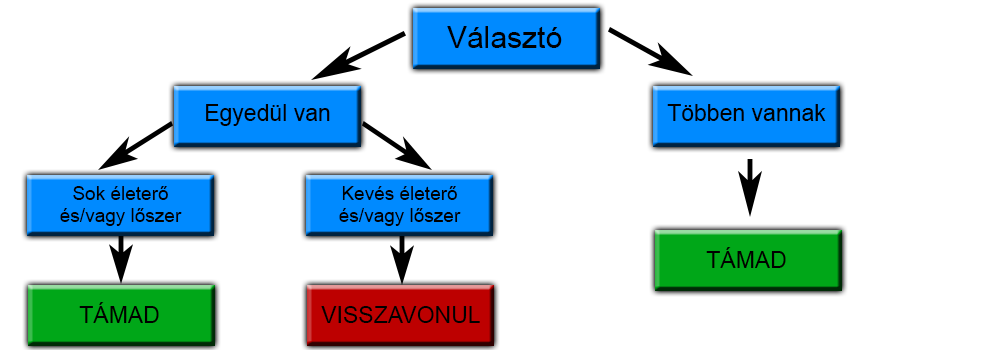
\includegraphics[scale=0.38]{kepek/viselkedes.png}
\caption{Az ellenfél egy lehetséges viselkedése}
\label{fig:behavior}
\end{figure}

\subsubsection{Adott ellenfél karakterisztikája}

\begin{tabular}{r|l}
Név & Az ellenfél neve. \\
Támadóképesség & Ellenfél képességei támadás közben.\\
&> 0.0 \& < 0.15 = Nem mozdul.\\
&>= 0.15 \& < 0.5 = Csak előre és hátra mozog.\\
&>= 0.5 \& < 1.0 = Körbe-körbe megy.\\
&> 0.6 \& < 1.0 = Véletlenszerű mozgás irányváltással.\\
&> 0.4 \& < 1.0 = Visszavonuláskor is fedezze magát lövéssel.\\
Agresszió & Az ellenfél agressziója.\\
Neme & Férfi, nő, vagy egyéb teremtmény\\
Célzóképesség & Fegyverenként különbözhet.\\
&> 0.0 \& < 0.9 = Az ellenfél mozgása hatással van a célzásra.\\
&> 0.4 \& <= 0.8 = Ellenfélmozgás követése.\\
&> 0.8 \& <= 1.0 = Várható felbukkanás helyének figyelése.\\
&> 0.6 \& <= 1.0 = Környezeti elemek felhasználása sebzésre.\\
Guggolás & Guggolás gyakorisága.\\
Ugrás & Ugrás gyakorisága.\\
Forgás & Forgás sebessége (reflex).\\
Reakcióidő & Miután meglát, mennyi idő telik el az első lövésig.\\
Lövéspontosság & 0 és 1 közötti érték, a lövés szórását adja meg.\\
Bosszú & Az ellenfél bosszúállósága\\
\end{tabular}

\subsection{Kimenetek}

A bemeneti adatok alapján a program egy modulja kiértékeli az eseményeket, és annak kimeneti értékei határozzák meg a következményeket.

